\documentclass[border=6pt]{standalone}
\usepackage{amsmath,amssymb}
\usepackage{xcolor}
\usepackage{tikz}
\usetikzlibrary{arrows.meta,backgrounds}
\definecolor{cblue}{HTML}{1976D2}
\definecolor{cred}{HTML}{E53935}
\definecolor{cpurple}{HTML}{5E35B1}
\definecolor{cgrey}{HTML}{757575}
\tikzset{every picture/.append style={show background rectangle,
    background rectangle/.style={fill=white}, inner frame sep=4pt}}
\newcommand{\bu}{\mathbf{u}}
% A near recurrence: the trajectory leaves u(t) and comes back close to a shifted copy of it.
\begin{document}
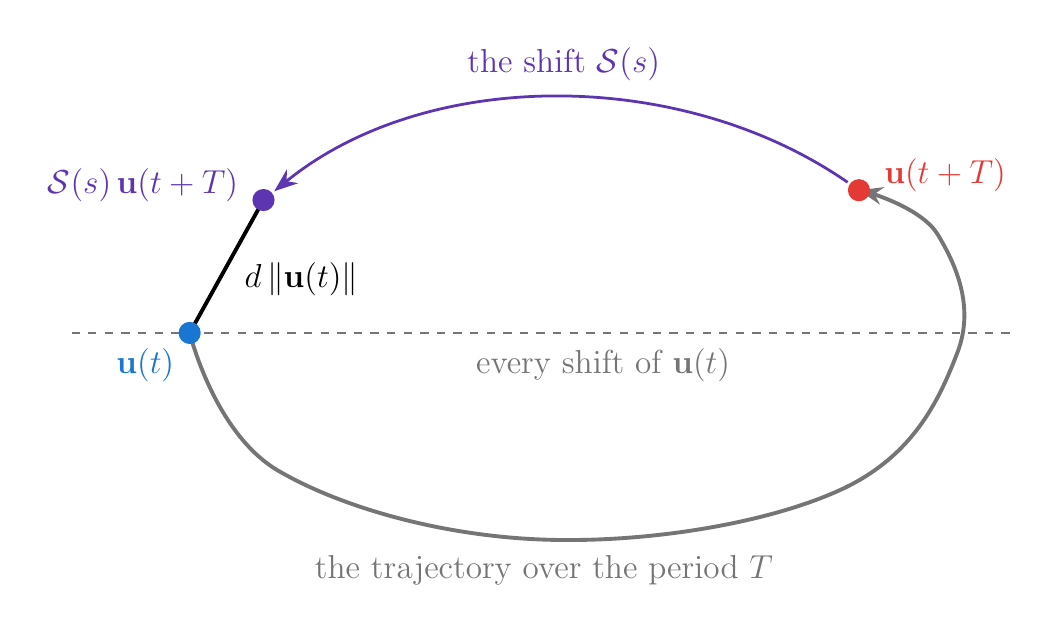
\begin{tikzpicture}[>={Stealth[length=3mm]}, every node/.style={font=\large}, x=1.25cm, y=1.25cm,
                    line width=1pt]
  % ---- the copies of the start under every shift ----
  \draw[cgrey, dashed] (-1.2, 0) -- (8.4, 0);
  \node[cgrey, below] at (4.2, -0.05) {every shift of $\bu(t)$};

  % ---- the trajectory over the period, below the copies and back above them ----
  \draw[cgrey, line width=1.4pt, ->] plot[smooth, tension=0.65] coordinates
      {(0, 0) (0.9, -1.4) (3.6, -2.1) (6.6, -1.6) (7.8, -0.2) (7.6, 1.0) (6.8, 1.45)};
  \node[cgrey, below] at (3.6, -2.15) {the trajectory over the period $T$};

  % ---- the start, the end, and the end shifted back near the start ----
  \draw[cpurple, ->, shorten >=5pt, shorten <=5pt] (6.8, 1.45) .. controls (5.0, 2.7) and (2.4, 2.7) .. (0.75, 1.35);
  \node[cpurple, above] at (3.8, 2.45) {the shift $\mathcal{S}(s)$};
  \draw[black, line width=1.4pt] (0, 0) -- (0.75, 1.35);
  \node[black, right] at (0.45, 0.55) {$d\,\|\bu(t)\|$};
  \fill[cblue] (0, 0) circle (4pt);
  \node[cblue, below left] at (-0.05, -0.05) {$\bu(t)$};
  \fill[cred] (6.8, 1.45) circle (4pt);
  \node[cred, right] at (6.95, 1.6) {$\bu(t + T)$};
  \fill[cpurple] (0.75, 1.35) circle (4pt);
  \node[cpurple, left] at (0.6, 1.5) {$\mathcal{S}(s)\,\bu(t + T)$};
\end{tikzpicture}
\end{document}
